\documentclass[12pt]{article}
\usepackage[paper=letterpaper,margin=2.5cm]{geometry}
\usepackage{amsmath,amssymb,amsfonts}
\usepackage{newtxtext, newtxmath}
\usepackage{enumitem}
\usepackage{titling}
\usepackage[colorlinks=true]{hyperref}
\usepackage{multirow}
\usepackage{svg}
\usepackage{listings}
\usepackage{xcolor}
\usepackage{float}

\setlength{\droptitle}{-6em}

\definecolor{codegreen}{rgb}{0,0.6,0}
\definecolor{codegray}{rgb}{0.5,0.5,0.5}
\definecolor{codepurple}{rgb}{0.58,0,0.82}
\definecolor{backcolour}{rgb}{0.95,0.95,0.92}

\lstdefinestyle{mystyle}{
    commentstyle=\color{codegreen},
    keywordstyle=\color{magenta},
    numberstyle=\tiny\color{codegray},
    stringstyle=\color{codepurple},
    basicstyle=\ttfamily\footnotesize,
    breakatwhitespace=false,
    breaklines=true,
    captionpos=b,
    keepspaces=true,
    numbers=left,
    numbersep=5pt,
    showspaces=false,
    showstringspaces=false,
    showtabs=false,
    tabsize=2
}
\lstset{style=mystyle}

\begin{document}

\begin{center}
\large{Aprendizagem 2023}\\
Homework I -- Group 28\\
\vskip 0.3cm
Gonçalo Bárias (ist1103124) \& Raquel Braunschweig (ist1102624)\vskip 1cm

\large{\textbf{Part I}: Pen and Paper}\normalsize
\end{center}

\noindent Consider the partially learnt decision tree from the dataset $D$. $D$ is described by four input variables –
one numeric with values in $[0,1]$ and 3 categorical – and a target variable with three classes.

\begin{figure}[H]
    \centering
    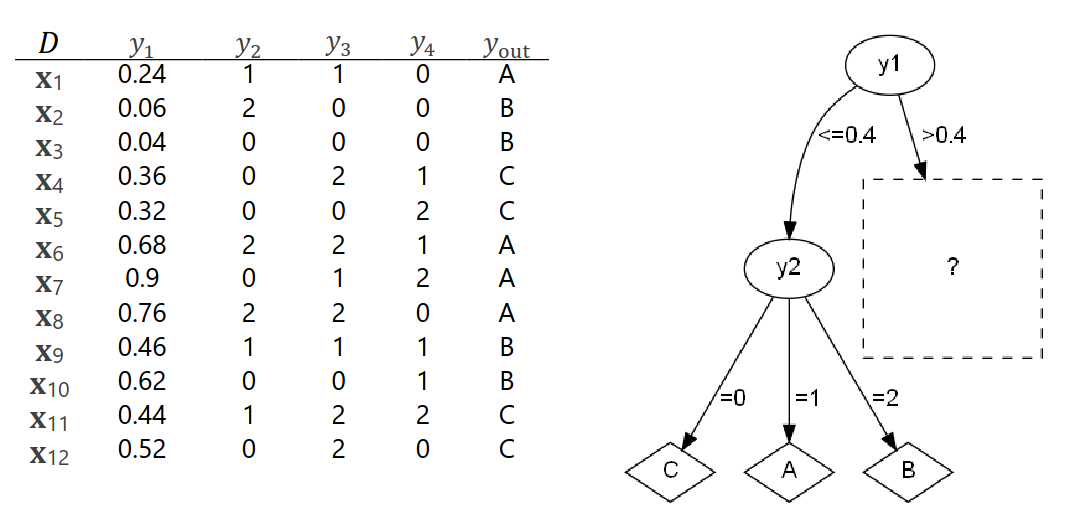
\includegraphics[width=15cm]{./assets/partial_tree_dataset_d}
    \caption{Partially Learnt Decision Tree and Dataset $D$ from Part I}
    \label{fig:PartI-partial-decision-tree-dataset-d}
\end{figure}

\begin{enumerate}[leftmargin=\labelsep]
    \item \textbf{Complete the given decision tree using Information gain with Shannon entropy ($log_2$).
    Consider that: i) a minimum of 4 observations is required to split an internal node, and
    ii) decisions by ascending alphabetic order should be placed in case of ties.}

    The entropy of \(y_{out}\) is given by:

    \begin{equation}
        \begin{split}
            E(y_{out} |y_1 > 0.4) = \quad
            & \quad  p(\text{A}, y_1 > 0.4) \log_2 \left(p(\text{A}, y_1 > 0.4)\right)  \\
            & + p(\text{B}, y_1 > 0.4) \log_2 \left(p(\text{B}, y_1 > 0.4)\right) \\
            & + p(\text{C}, y_1 > 0.4) \log_2 \left(p(\text{C}, y_1 > 0.4)\right) \\
        \end{split}
    \end{equation}

    We can calculate $E(y_{out})$:

    \[
        \begin{aligned}
            E(y_{out}) & = - \left(\frac{3}{7} \log_2\left(\frac{3}{7}\right) + \frac{2}{7} \log_2\left(\frac{2}{7}\right) 
                            + \frac{2}{7} \log_2\left(\frac{2}{7}\right)\right) \\
                       & = 1.5567
        \end{aligned}
    \]
     
    \newpage

    The next step is calculating $E(y_{out} | y_1 > 0.4 , y_x)$, in which x will take the values of 2, 3 or 4:

    \begin{equation}\label{exI1-e-yout-y2}
        \begin{split}
            E(y_{out} |y_1 > 0.4 , y_x) = \quad
            & \quad  p(y_x = 0) E(y_{out} | y_x > 0.4 , y_2 = 0) \\
            & + p(y_x = 1) E(y_{out} | y_x > 0.4 , y_2 = 1) \\
            & + p(y_x = 2) E(y_{out} | y_x > 0.4 , y_2 = 2)
        \end{split}
    \end{equation}

    And the information gain of variable $y_x$ is given by

    \begin{equation}\label{ex1-ig}
        IG(y_x) = E(y_{out}) - E(y_{out} |y_1 > 0.4, y_x)
    \end{equation}


    \textbf{Let's start with x = 2}:

    \[
        \begin{aligned}
            p(y_2 = 0, y_1 > 0.4)          & = \frac{3}{7}                                                                                               \\
            p(y_2 = 1, y_1 > 0.4)          & = \frac{2}{7}                                                                                              \\
            p(y_2 = 1, y_1 > 0.4)          & = \frac{2}{7}                                                                                              \\
            E(y_{out} | y_x > 0.4 , y_2 = 0) & = - \left(\frac{1}{3} \log_2\left(\frac{1}{3}\right) + \frac{1}{3} \log_2\left(\frac{1}{3}\right) 
                + \frac{1}{3} \log_2\left(\frac{1}{3}\right)\right) = 1.5849                                                                   \\
            E(y_{out} | y_x > 0.4 , y_2 = 1) & = - \left(\frac{0}{2} \log_2\left(\frac{0}{2}\right) + \frac{1}{2} \log_2\left(\frac{1}{2}\right) 
                + \frac{1}{2} \log_2\left(\frac{1}{2}\right)\right) = 1                                                                        \\
            E(y_{out} | y_x > 0.4 , y_2 = 2) & = - \left(\frac{2}{2} \log_2\left(\frac{2}{2}\right) + \frac{0}{2} \log_2\left(\frac{0}{2}\right) 
                + \frac{0}{2} \log_2\left(\frac{0}{2}\right)\right) = 0                  
        \end{aligned}
    \]

    Therefore, replacing these values on equation \eqref{exI1-e-yout-y2}, gives us:

    \[
        \begin{aligned}
            E(y_{out} | y_1>0.4, y_2) & = \frac{3}{7} \times 1.5849 + \frac{2}{7} \times 1 +  \frac{2}{7} \times 0\\
                             & = 0.965.
        \end{aligned}
    \]

    Finally, we can calculate the information gain, as per \eqref{ex1-ig},

    \[
        IG(y_{2}) = 1.5567 - 0.965 = 0.5917
    \]
    
    \newpage
    \textbf{Now, let's calculate for x = 3}:

    \[
        \begin{aligned}
            p(y_3 = 0, y_1 > 0.4)          & = \frac{1}{7}                                                                                    \\
            p(y_3 = 1, y_1 > 0.4)          & = \frac{2}{7}                                                                                    \\
            p(y_3 = 2, y_1 > 0.4)          & = \frac{4}{7}                                                                                    \\
            E(y_{out} | y_x > 0.4 , y_3 = 0) & = - \left(\frac{0}{1} \log_2\left(\frac{0}{1}\right) + \frac{1}{1} \log_2\left(\frac{1}{1}\right) 
                + \frac{0}{1} \log_2\left(\frac{0}{1}\right)\right) = 0                                                                       \\
            E(y_{out} | y_x > 0.4 , y_3 = 1) & = - \left(\frac{1}{2} \log_2\left(\frac{1}{2}\right) + \frac{1}{2} \log_2\left(\frac{1}{2}\right) 
                + \frac{0}{2} \log_2\left(\frac{0}{2}\right)\right) = 1                                                                       \\
            E(y_{out} | y_x > 0.4 , y_3 = 2) & = - \left(\frac{2}{4} \log_2\left(\frac{2}{4}\right) + \frac{0}{4} \log_2\left(\frac{0}{4}\right) 
                + \frac{2}{4} \log_2\left(\frac{2}{4}\right)\right) = 1                  
        \end{aligned}
    \]

    Therefore, replacing these values on equation \eqref{exI1-e-yout-y2}, gives us:

    \[
        \begin{aligned}
            E(y_{out} | y_1>0.4, y_3) & = \frac{1}{7} \times 0 + \frac{2}{7} \times 1 +  \frac{4}{7} \times 1                                \\
                             & = 0.8571.
        \end{aligned}
    \]

    Finally, we can calculate the information gain, as per \eqref{ex1-ig},

    \[
        IG(y_{3}) = 1.5567 - 0.8571 = 0.6996 
    \]

    \textbf{Finally, let's calculate for x = 4}:

    \[
        \begin{aligned}
            p(y_4 = 0, y_1 > 0.4)          & = \frac{2}{7}                                                                                     \\
            p(y_4 = 1, y_1 > 0.4)          & = \frac{3}{7}                                                                                     \\
            p(y_4 = 1, y_1 > 0.4)          & = \frac{2}{7}                                                                                     \\
            E(y_{out} | y_x > 0.4 , y_4 = 0) & = - \left(\frac{1}{2} \log_2\left(\frac{1}{2}\right) + \frac{0}{2} \log_2\left(\frac{0}{2}\right) 
                + \frac{1}{2} \log_2\left(\frac{1}{3}\right)\right) = 1                                                                   \\
            E(y_{out} | y_x > 0.4 , y_4 = 1) & = - \left(\frac{1}{3} \log_2\left(\frac{1}{3}\right) + \frac{2}{3} \log_2\left(\frac{2}{3}\right) 
                + \frac{0}{3} \log_2\left(\frac{0}{3}\right)\right) = 0.9183                                                                       \\
            E(y_{out} | y_x > 0.4 , y_4 = 2) & = - \left(\frac{1}{2} \log_2\left(\frac{1}{2}\right) + \frac{0}{2} \log_2\left(\frac{0}{2}\right) 
                + \frac{1}{2} \log_2\left(\frac{1}{2}\right)\right) = 1                  
        \end{aligned}
    \]

    Therefore, replacing these values on equation \eqref{exI1-e-yout-y2}, gives us:

    \[
        \begin{aligned}
            E(y_{out} | y_1>0.4, y_4) & = \frac{2}{7} \times 1.5849 + \frac{3}{7} \times 1 +  \frac{2}{7} \times 0\\
                             & = 0.965.
        \end{aligned}
    \]

    Finally, we can calculate the information gain, as per \eqref{ex1-ig},

    \[
        IG(y_{4}) = 1.5849 - 0.965 = 0.5917
    \]
    
    
    \textbf{Upon computing the information gains for each attribute,} it is evident that $y_3$ yields the highest value of 0.6996. Consequently,
        it is selected as the next node, resulting in the construction of the following decision tree:

    Por arvore aqui (ns bem como fazer help)
    
    \item \textbf{Draw the training confusion matrix for the learnt decision tree.}

    Blah

    \item \textbf{Identify which class has the lowest training F1 score.}

    Blah

    \item \textbf{Considering $y_2$ to be ordinal, assess if $y_1$ and $y_2$ are correlated using the Spearman coefficient.}

    Blah

    \item \textbf{Draw the class-conditional relative histograms of $y_1$ using 5 equally spaced bins in $[0,1]$.
    Find the root split using the discriminant rules from these empirical distributions.}

    Blah
\end{enumerate}

\vskip 0.5cm

\begin{center}
\large{\textbf{Part II}: Programming}\normalsize
\end{center}

\noindent Consider the \texttt{column\_diagnosis.arff} data available at the homework tab, comprising 6 biomechanical
features to classify 310 orthopaedic patients into 3 classes (\texttt{normal}, \texttt{disk hernia}, \texttt{spondilolysthesis}).

\begin{enumerate}[leftmargin=\labelsep]
    \item \textbf{Apply \texttt{f\_classif} from \texttt{sklearn} to assess the discriminative power of the input variables.
          Identify the input variable with the highest and lowest discriminative power.
          Plot the class-conditional probability density functions of these two input variables.}

          \vskip 0.3cm
          \lstinputlisting[language=Python]{./assets/code_1.py}

          \vskip -0.8cm
          \begin{figure}[H]
              \centering
              \includesvg[width=14cm]{./assets/class_conditional_probability.svg}
              \caption{Class-conditional probability density functions of the highest and lowest discriminative power variables.}
              \label{fig:PartII-ex1-plot}
          \end{figure}

    \item \textbf{Using a stratified 70-30 training-testing split with a fixed seed (\texttt{random\_state=0}), assess in a
          single plot both the training and testing accuracies of a decision tree with depth limits in
          $\{1,2,3,4,5,6,8,10\}$ and the remaining parameters as default.\vskip 0.05cm
          \textit{[Optional]} Note that split thresholding of numeric variables in decision trees is non-deterministic
          in sklearn, hence you may opt to average the results using 10 runs per parameterization.}

          \vskip 0.3cm
          \lstinputlisting[language=Python]{./assets/code_2.py}

          \vskip -0.8cm
          \begin{figure}[H]
              \centering
              \includesvg[width=14cm]{./assets/training_testing_accuracies.svg}
              \caption{Accuracy of the trained decision tree, applied to both a test and training sets, for varying depth limits.}
              \label{fig:PartII-ex2-plot}
          \end{figure}

    \item \textbf{Comment on the results, including the generalization capacity across settings.}

          Blah
    
    \newpage
    
    \item \textbf{To deploy the predictor, a healthcare team opted to learn a single decision tree
          (\texttt{random\_state=0}) using \textit{all} available data as training data, and further ensuring that each leaf has
          a minimum of 20 individuals in order to avoid overfitting risks.}
          \begin{enumerate}
          \item \textbf{Plot the decision tree.}

          \vskip -0.5cm
          \begin{figure}[H]
              \centering
              \includesvg[width=14cm]{decision_tree.svg}
              \caption{Accuracy of trained decision tree, applied to both a test and training sets, for varying depth limits.}
              \label{fig:PartII-ex2-plot}
          \end{figure}

          \item \textbf{Characterize a hernia condition by identifying the hernia-conditional associations.}

          Blah
          \end{enumerate}
\end{enumerate}

\vskip 1cm
\center\textbf{END}

\end{document}
